% -*- root: ../../main.tex -*-
%!TEX root = ../../main.tex

\graphicspath{{chapters/layer_opt/figures/}}
% ----------------------- contents from here ------------------------

\chapter{Model-based Design Of Pouch Cells}\label{ch:modelbaseddesign}
\vspace*{-1em}
\startcontents[chapters]
\printcontents[chapters]{}{1}{\setcounter{tocdepth}{1}}

\bigskip

\begin{figure}[!bp]
    \begin{minipage}[t]{\textwidth}
        \centering
        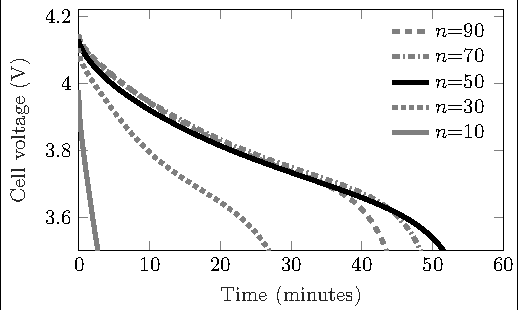
\includegraphics[trim=4 4 2 4,clip]{fig_CC_discharge_curves.pdf}
        \caption
        [%
        Voltage  curves   for  a   \SI{60}{\ampere}  galvanostatic   discharge  from
        \SI{100}{\percent} \glsfmtshort{soc}  until cut-off voltage for  a few layer
        choices, in a pouch cell of fixed exterior height.
        ]%
        {%
            Terminal  voltage   curves  of   a  Li-ion  cell   (with  parameters
            given in  \cref{tbl:lcoSimParamslayeropt}) under  a \SI{60}{\ampere}
            galvanostatic    discharge    beginning   from    \SI{100}{\percent}
            \glsfmtshort{soc}  until  lower  cut-off  voltage for  a  few  layer
            choices~$n$, in a  pouch cell of fixed exterior  height. The maximum
            usable  energy  is  achieved  for  an  intermediate  choice  of  $n$
            that  corresponds  to neither  the  highest  nominal capacity  layer
            configuration ($n$=\num{10}) nor the  highest electrode surface area
            configuration ($n$=\num{90})\footnotemark.
        }%
        \label{fig:fig_CC_discharge_curves}
        \mpfootnotes[1]
        \footnote{This figure was created by Ian Campbell who asserts copyright,
            with  intellectual  contributions  from  and   the  right  to  use  asserted  by
        Krishnakumar Gopalakrishnan.}
    \end{minipage}
\end{figure}

% -*- root: ../../main.tex -*-
%!TEX root = ../../main.tex

\begin{table}[!htbp]
    \caption
    [%
    Theoretical  capacity \&  usable energy  of a  Li-ion cell  for a  few layer
    choices under a \SI{60}{\ampere} galvanostatic discharge
    ]
    {%
        Theoretical capacity and usable energy of a Li-ion cell (with parameters
        given in \cref{tbl:lcoSimParamslayeropt}) for  a few layer choices under
        a \SI{60}{\ampere} galvanostatic discharge.
    }%
    \label{tbl:CC_discharge_curves_table}
    \centering
    \begin{tabular}{@{} S[table-format=2.0] S[table-format=1.2] S[table-format=2.2]  S[table-format=3.2] S[table-format=2.2] @{}}
        \toprule
        \multicolumn{1}{@{} l}{$n$} &  \multicolumn{1}{c}{\footnotesize C-rate} & \multicolumn{1}{c}{\footnotesize \makecell{Theoretical \\ Capacity  (\si{Ah})}} & \multicolumn{1}{c}{\footnotesize \makecell{Usable \\ Energy \si{(Wh)}}} & \multicolumn{1}{c @{}}{\footnotesize \makecell{Remaining \\ SOC  (\si{\percent})}} \\
        \midrule
        90 & 1.24 & 48.25 & 166.46 & 9.84  \\
        70 & 1.11 & 53.99 & 184.80 & 10.26 \\
        50 & 1.00 & 59.73 & 195.47 & 13.51 \\
        30 & 0.92 & 65.47 & 101.20 & 58.95 \\
        10 & 0.84 & 71.21 & 10.15  & 96.22 \\
        \bottomrule
    \end{tabular}
\end{table}


\begin{figure}[!bp]
    \begin{minipage}[t]{\textwidth}
        \centering
        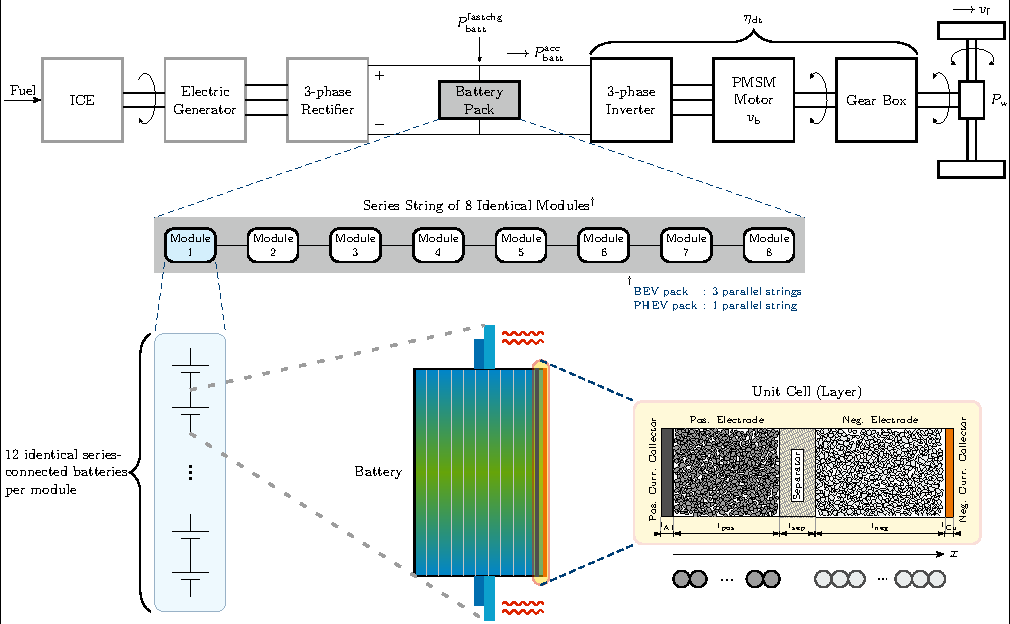
\includegraphics[width=\textwidth]{hierarchical_powertrain_to_cell_layer.pdf}
        \caption
        [%
        Vehicle-to-cell hierarchical  overview of  an electrified powertrain architecture.
        ]%
        {%
            Schematic  depicting   the  vehicle-to-cell  hierarchical   overview  of
            a  typical   electrified  powertrain   architecture.  This   represents  the
            system-level context within which  the proposed layer optimisation framework
            has been developed. Two \glsfmtshort{xeV} powertrains ---
            \begin{enumerate*}[label=\itshape\alph*\upshape)]
                \item  a \gls{bev}, and
                \item  a series \gls{phev}
            \end{enumerate*}
            are  chosen as  examples  to demonstrate  how  the methodology  facilitates
            common module designs for such battery packs\footnotemark.
        }%
        \label{fig:fig_PowertrainSchematic}
        \mpfootnotes[1]
        \footnote{This  figure was  created by  Krishnakumar Gopalakrishnan  who
            asserts copyright, with intellectual contributions from and the right to
        use asserted by Ian Campbell.}
    \end{minipage}
\end{figure}

\begin{figure}[p]
    \begin{minipage}[t]{\textwidth}
        \centering
        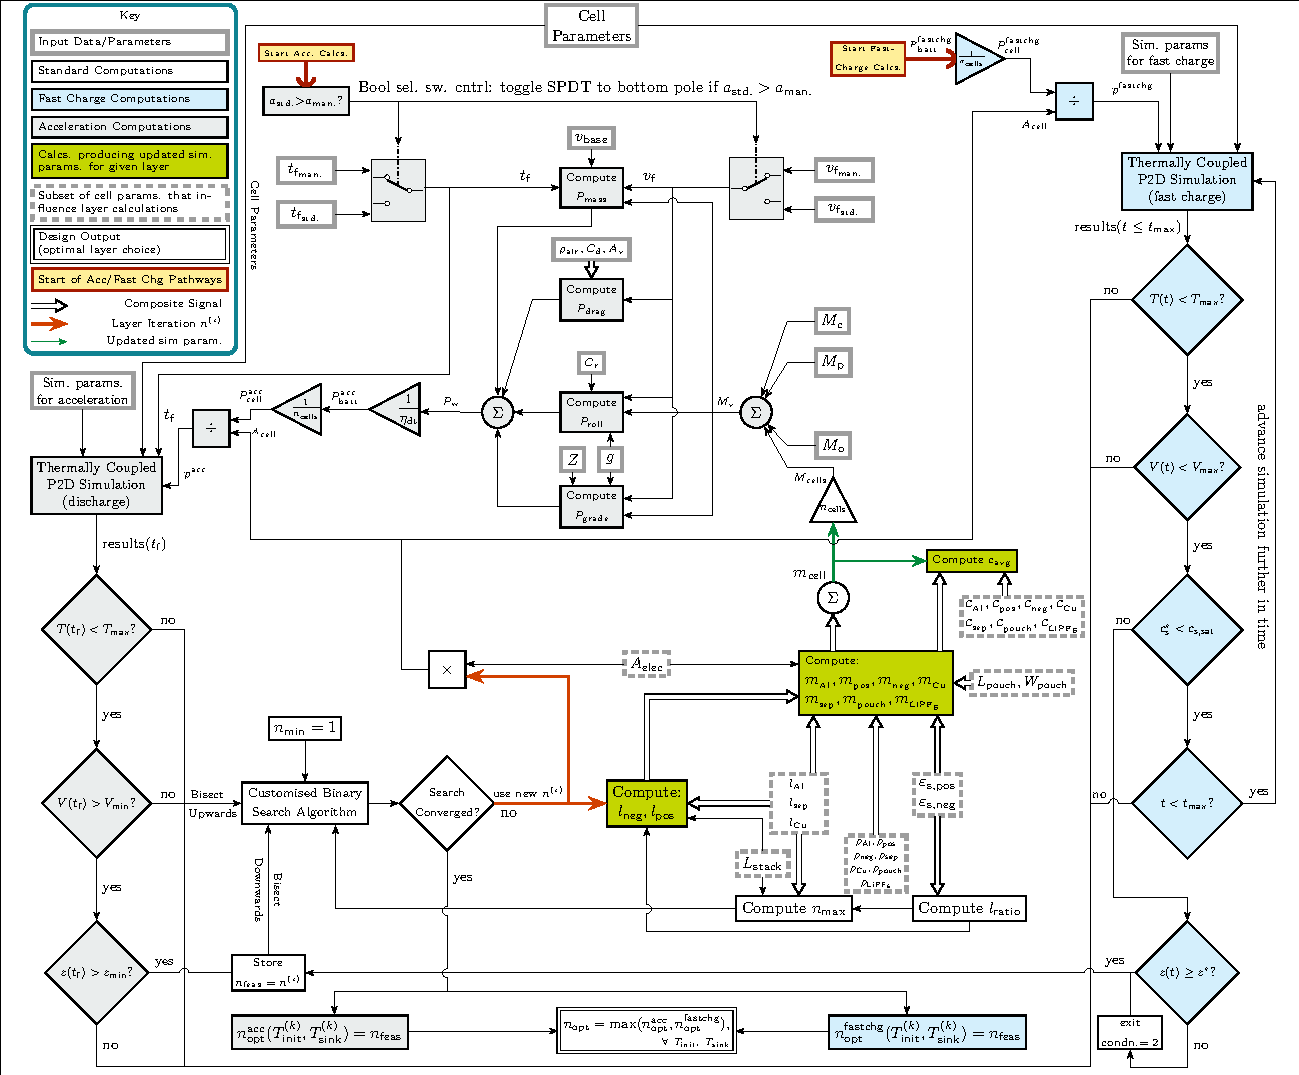
\includegraphics[angle=90, width=\textwidth]{fig_master_flow_diagram}
        \caption
        [%
        Flow diagram depicting an overview  of the proposed layer optimisation methodology
        for Li-ion pouch cells.
        ]%
        {%
            Flow diagram depicting an overview  of the proposed layer optimisation methodology
            for Li-ion pouch cells\footnotemark.
        }%
        \label{fig:fig_strategy_schematic}
        \mpfootnotes[1]
        % \vspace*{1.125cm}
        \vspace*{0.7225cm}
        \footnote{This  figure was  created by  Krishnakumar Gopalakrishnan  who
            asserts copyright, with intellectual contributions from and the right to
        use asserted by Ian Campbell.}
    \end{minipage}
\end{figure}

\section{Lower Cutoff Voltage}\label{sec:cutoff}
% -*- root: ../../main.tex -*-
%!TEX root = ../../main.tex
% vim:nospell

\begin{table}[!htbp]
    \small
    \caption[%
    System-level simulation conditions \& thermal parameters of  an \glsfmtshort{lco} cell
    ]%
    {%
        Cell   parameters   and   system   conditions  for   a   simulating   an
        \glsfmtshort{lco} cell  with the  \gls{dfn} electrochemical model  and a
        lumped thermal model. The parameters  presented here when augmented with
        the  values  of  the  kinetic, geometric  and  transport  properties  of
        the  cell (from  \cref{tbl:lcoSimParamsSPMp2d}  represents the  complete
        information  required for  all  simulations in  this layer  optimisation
        framework.
    }%
    \label{tbl:lcoSimParamslayeropt}
    \vspace{-2.6229525pt}
    \begin{threeparttable}
        \centering
        \textbf{System Conditions} \\ \smallskip
        \begin{varwidth}[t]{0.48\linewidth}
            \begin{tabular*}{\textwidth}{@{} l @{\extracolsep{\fill}} S[table-format=1.2,table-space-text-pre=\Tnote{a} ,table-align-text-pre=false] @{}}
                \toprule
                \multicolumn{1}{@{}l}{Parameter} \\
                \midrule

                Lower cutoff cell voltage, $V_\text{min}$ (\si{\volt}) & \Tnote{a} 3.50   \\
                Upper cutoff cell voltage, $V_\text{max}$ (\si{\volt}) & \Tnote{b} 4.22   \\

                \bottomrule
            \end{tabular*}
        \end{varwidth}
        \hfill
        \begin{varwidth}[t]{0.48\linewidth}
            \begin{tabular*}{\textwidth}{@{} l @{\extracolsep{\fill}} S[table-format=2.2,table-space-text-pre=\Tnote{a} ,table-align-text-pre=false] @{}}
                \toprule
                \multicolumn{1}{@{}l}{Parameter} \\
                \midrule

                Target cell SOC for fast charge, $z^\ast$ \si{(\%)}                & \Tnote{c} 80.00 \\
                Cell upper temperature limit, $T_\text{max}$ \si{(\degreeCelsius)} & \Tnote{d} 55.00 \\

                \bottomrule
            \end{tabular*}
        \end{varwidth}

        \medskip
        \begin{tabular*}{\textwidth}{@{} l @{\extracolsep{\fill}} r @{}}
            \multicolumn{2}{c}{\textbf{Geometric Parameters}} \\
            \toprule
            \multicolumn{1}{@{}l}{Parameter} \\
            \midrule
            Surface area of pos.\ \& neg.\ electrode overlap within a layer, {$A_\text{elec}$} \si{(m^2)} & \textsuperscript{b}\num{4.19e-2}   \\
            Exterior pouch length, $L_\text{pouch}$ \si{(m)}                                              & \textsuperscript{e}\num{332.74e-3} \\
            Exterior pouch width, $W_\text{pouch}$ \si{(m)}                                               & \textsuperscript{e}\num{99.06e-3}  \\
            Exterior pouch height, $H_\text{pouch}$ \si{(m)}                                              & \textsuperscript{f}\num{10.00e-3}  \\
            Pouch material thickness, $T_\text{pouch}$ \si{(m)}                                           & \textsuperscript{g}\num{160.00e-6} \\
            \bottomrule
        \end{tabular*}
        \medskip
        \centering \textbf{Thermal Parameters} \\ \smallskip
        \resizebox{\textwidth}{!}{%
            \begin{tabular}{@{} l S[table-format=4.0,table-space-text-pre=\Tnote{m} ,table-align-text-pre=false] S[table-format=4.1,table-space-text-pre=\Tnote{m} ,table-align-text-pre=false] S[table-format=4.1,table-space-text-pre=\Tnote{m} ,table-align-text-pre=false] S[table-format=4.2,table-space-text-pre=\Tnote{m} ,table-align-text-pre=false] S[table-format=4.0,table-space-text-pre=\Tnote{m} ,table-align-text-pre=false] S[table-format=4.1,table-space-text-pre=\Tnote{m} ,table-align-text-pre=false] S[table-format=4.1,table-space-text-pre=\Tnote{m} ,table-align-text-pre=false] @{}}
                \toprule
                \multicolumn{1}{@{}l}{Parameter} & \multicolumn{1}{c}{Al.\ CC} & \multicolumn{1}{c}{Pos} & \multicolumn{1}{c}{Sep} & \multicolumn{1}{c}{Neg} & \multicolumn{1}{c}{Cu.\ CC} & \multicolumn{1}{c}{\ch{LiPF_6}} & \multicolumn{1}{r@{}}{Pouch}\\
                \midrule

                Sp.\ heat capacity, $c_j$ (\si{\joule\per\kilogram\per\kelvin})   & \Tnote{h} 903  & \Tnote{h} 1269.2 & \Tnote{h} 1978.2 & \Tnote{h} 1437.4 & \Tnote{h} 385  & \Tnote{h} 2055.1 & \Tnote{i} 1464.8 \\
                Density, $\rho_j$ (\si{\kilogram\per\meter\cubed})                & \Tnote{j} 2700 & \Tnote{k} 2291.6 & \Tnote{b} 1100.0 & \Tnote{j} 2660.0 & \Tnote{l} 8960 & \Tnote{j} 1290.0 & \Tnote{m} 1150.0 \\
                Activ.\ energy, diff. ${E_\text{act,s}}_j$ (\si{\joule\per\mole}) & {---}                   & \Tnote{p} 5000   & {---}                     & \Tnote{p} 5000   & {---}                   & {---}                     & \multicolumn{1}{c}{---}   \\
                Activ.\ energy, rxn. ${E_\text{act,k}}_j$ (\si{\joule\per\mole})  & {---}                   & \Tnote{p} 5000   & {---}                     & \Tnote{p} 5000   & {---}                   & {---}                     & \multicolumn{1}{c}{---}   \\

                \bottomrule
            \end{tabular}
        }
        \medskip
        \begin{tabular*}{\textwidth}{@{} l @{\extracolsep{\fill}} r @{}}
            \multicolumn{2}{c}{\textbf{Other Geometric/Cell-Level Parameters}} \\
            \toprule
            \multicolumn{1}{@{}l}{Parameter} \\
            \midrule

            Thickness of pos.\ current collector, $l_\text{Al}$ \si{(m)}                    & \textsuperscript{f}\num{15e-6}   \\
            Thickness of neg.\ current collector, $l_\text{Cu}$ \si{(m)}                    & \textsuperscript{p}\num{10e-6}   \\
            Total tab area, $A_\text{tabs}$ \si{(m^2)}                                      & \textsuperscript{b}\num{5.94e-3} \\
            Lumped heat transfer coefficient, $h$ (\si{\watt\per\meter\squared\per\kelvin}) & \textsuperscript{b}150           \\
            Initial electrolyte concentration, $c_\text{e,0}$ (\si{\mole\per\meter\cubed})  & \textsuperscript{q}1000          \\

            \bottomrule
        \end{tabular*}

        \medskip
        \begin{tabular*}{\textwidth}{@{} =P{7.5cm}  +l@{\extracolsep{\fill}}+c +r @{}}
            \multicolumn{4}{c}{\textbf{Spatial Discretisation}} \\
            \toprule
            \multicolumn{1}{@{}l}{Parameter} & \multicolumn{1}{l}{Pos} & \multicolumn{1}{c}{Sep} & \multicolumn{1}{r@{}}{Neg}\\
            \midrule

            Nodes, through-thickness (axial), $N_{\text{a}_j}$          & \num{40} & \num{40} & \num{40} \\
            Nodes, within spherical particle (radial), $N_{\text{r}_j}$ & \num{15} & ---      & \num{15} \\

            \bottomrule
        \end{tabular*}

        \medskip
        \vspace{-2.6229525pt}
        \begin{tablenotes}[para,flushleft]
            \begin{footnotesize}
            \item[a] Calculated as described in \cref{sec:cutoff}
            \item[b] Assumed
            \item[c] Ref.~\cite{Sae2010}
            \item[d] Ref.~\cite{Kizilel2009} \\
            \item[e] Converted from imperial units reported in~Ref.~\cite{GMBoltBatteryDims}
		    \item[f] Table~\romanletter{4} of~Ref.~\cite{Groger2015} \\
            \item[g] Sum of values in table~1 of~Ref.~\cite{Svens2013}
            \item[h] Ref.~\cite{Chen2005}
            \item[i] Computed from values of constituents (see~\cite{Svens2013}) using Ref.~\cite{martienssen2006springer} \\
            \item[j] Ref.~\cite{Guo2010}
            \item[k] Ref.~\cite{Jeon2011}
            \item[l] Ref.~\cite{Worwood2017,Song2000}
            \item[m] Ref.~\cite{Kim2009}
            \item[p] Ref.~\cite{Northrop2011}
            \item[q] Ref.~\cite{Subramanian2009}
            \end{footnotesize}
        \end{tablenotes}
    \end{threeparttable}
\end{table}



Figure showing power input

\section{Hybrid Spectral-\glsfmtshort{fv} Scheme}\label{sec:hybridfv-spectral}

Fast  and  accurate  estimation  of   the  solid  phase  lithium  concentration,
particularly  its   value  at   the  surface  of   electrode  particles   is  an
inherent  requirement   of  the   layer  optimisation  procedure   presented  in
Section~\ref{sec:Framework}. The high power densities that result from using low
layer  counts  necessitate  this  requirement. It  has  been  acknowledged  that
concentration  calculations employing  polynomial approximations  such as  those
proposed in~\cite{Santhanagopalan2006a}  lack fidelity at  high charge/discharge
rates~\cite{Santhanagopalan2006}.  Hence,  a  conventional  full-order  solution
based on Fick's law of diffusion is appropriate.

With full-order  solid phase  diffusion dynamics,  applying the  \gls{fv} scheme
(that has  been employed to  discretise all through-thickness \gls{pde}s  in the
\gls{p2d} model)  results in  a large system  of equations. This  is due  to the
requirement  of  using  a  high  radial  node  density  per  spherical  particle
for  improved  accuracy.  Consequently,  the  computational  cost  is  high  and
simulation  runtime  becomes prohibitive  when  exploring  the search  space  of
all  possible  layer configurations.  Moreover,  with  a cell-centered  \gls{fv}
discretisation,  it is  non-trivial to  directly apply  the ionic  flux boundary
condition  at the  particle surface,  since  it involves  extrapolation from  at
least  two  other nodes  within  the  particle.  While such  extrapolations  are
acceptable  in the  axial dimension  --- particularly  with high  node densities
providing  small values  of $\frac{\Delta  x}{2}$  --- they  are undesirable  in
the  radial  dimension.  This  is  because  cell's  open  circuit  and  terminal
voltages strongly depend on the  concentration at the particle surface. Spectral
methods  offer  a  combination  of  high accuracy  and  speed  while  permitting
the  use of  a  lower number  of  radial discretisation  nodes.  To implement  a
spectral  scheme on  a non-periodic  domain, a  Chebyshev discretisation  may be
applied~\cite{Trefethen2000}.  Bizeray~\etal discretised  all  of the  \gls{p2d}
model equations using this approach~\cite{Bizeray2015a}. However, this entails a
bi-directional  mapping of  all  variables between  the  physical and  Chebyshev
domains, incurring computational overhead.

Here we propose the use of a hybrid formulation of the \gls{p2d} model wherein a
standard \gls{fv}  scheme in the  axial dimension and  a spectral scheme  in the
radial domain  are used. By exploiting  the natural separation of  the axial and
radial  domains, we  \romanletter{1}) retain  the ability  to easily  couple the
molar  flux  density  at  the  particle surface  through  reformulation  of  the
boundary conditions  of the solid  diffusion pde and \romanletter{2})  solve for
solid-phase lithium concentration in the  Chebyshev domain and locally transform
to  physical domain,  without  requiring  system-wide Chebyshev  reformulations.
Although  the  proposed  implementation  does not  globally  employ  a  spectral
scheme, the  combined beneficial  effects of  radial-domain spectral  scheme and
automatic differentiation of system equations using CasADi~\cite{Andersson2013b}
facilitates rapid simulation, enabling  layer optimisation on short time-scales.
Eqns\cref{eqn:defineChebNodes}--\cref{eqn:solidDiffEqChebDomain}  detail the
steps  leading to  the reformulated  solid  phase diffusion  and its  associated
boundary condition in the Chebyshev domain.

The Chebyshev collocation nodes defined on a 1D mesh in the radial direction are
given by\cref{eqn:defineChebNodes}~\cite{Trefethen2000}.

\begin{equation}\label{eqn:defineChebNodes}
    \tilde{r} = \cos\left(\frac{i\pi}{N_\text{r}}\right), \qquad i = 0, 1, \dots  N_\text{r} \quad \tilde{r} \in [-1, 1]
\end{equation}

Assuming  constant diffusivity,  and expanding  the derivative  in the  standard
form   of  the   Fickian  spherical   diffusion  equation   for  each   particle
(refer~\ref{sec:Supplementary})  we  obtain  \cref{eqn:quotientappliedpde},
presented along  with its  Neumann boundary  conditions. $j$  is the  molar flux
density  (\si{mol.m^{-2}.s^{-1}})  and  $R_\text{p}$ is  the  particle  radius
(\si{m}).

\begin{align}
    \frac{\partial c_\text{s}}{\partial t} &= D^\text{eff}_\text{s} \left( \frac{\partial}{\partial r} \frac{\partial c_\text{s}}{\partial r} + \frac{\partial^2 c_\text{s}}{\partial r^2} \right) \qquad r \in [0, R_\text{p}]\label{eqn:quotientappliedpde}\\
\frac{\partial c_\text{s}}{\partial r}\bigg\rvert_{r=0} &= 0\tag{\ref{eqn:quotientappliedpde}a}\\
    D^\text{eff}_\text{s}\frac{\partial c_\text{s}}{\partial r}\bigg\rvert_{r=R_\text{p}} &= {}-j\tag{\ref{eqn:quotientappliedpde}b}
\end{align}

{Mapping} $r \in [0,R_\text{p}] \mapsto \tilde{r} \in [-1, 1]$,
\begin{align}\label{mappingChebDomain}
    r = \frac{R_\text{p}}{2}(\tilde{r} + 1)
\end{align}

Applying  \cref{mappingChebDomain}   to  \cref{eqn:quotientappliedpde}
whilst    retaining    $c_\text{s}$    in   the    physical    space    yields
\cref{eqn:solidDiffEqChebDomain}.

\begin{align}
	\frac{\partial c_\text{s}}{\partial t} &= 4 \frac{D^\text{eff}_\text{s}}{R_\text{p}^2} \left( \frac{2}{\tilde{r} + 1} \frac{\partial c_\text{s}}{\partial \tilde{r}} + \frac{\partial^2 c_\text{s}}{\partial {\tilde{r}}^2} \right)\label{eqn:solidDiffEqChebDomain}\\
\frac{\partial c_\text{s}}{\partial \tilde{r}}\bigg\rvert_{\tilde{r}=-1} &= 0\tag{\ref{eqn:solidDiffEqChebDomain}a}\\
	2 \frac{D^\text{eff}_\text{s}}{R_\text{p}} \frac{\partial c_\text{s}}{\partial \tilde{r}}\bigg\rvert_{\tilde{r}=1} &= -j\tag{\ref{eqn:solidDiffEqChebDomain}b}
\end{align}

During  the iterative  solution process,  the spatial  gradients of  solid phase
lithium concentration in  \cref{eqn:solidDiffEqChebDomain} are not computed
through  an  explicit  differentiation   procedure,  but  instead  evaluated  by
pre-multiplying  the  concentration  values  at   the  collocation  nodes  by  a
Chebyshev  differentiation  matrix.  This  particular fact  is  responsible  for
the  inherent  reduction  of  simulation   runtime  achieved  by  introducing  a
spectral  method.  In the  modified  version  of  LIONSIMBA  used in  the  layer
optimisation methodology, differentiation matrices of suitable dimension as well
as  the Chebyshev  collocation nodes  are  generated using  the MATLAB  function
\texttt{cheb.m}~\cite{Trefethen2000}.

%Honour  code pledge:  This  chapter  plan was  written  without  looking at  the
%manuscript even  once. Only the actual  code commits of LIONSIMBA,  BOLD toolbox
%and the data from shared Box folder was used in writing this up.

%The literature review for this chapter shall be split over two parts - the first
%part shall be in a separate literature review chapter. The other part will be in
%this chapter,  but peppered in  multiple areas/sections. To clarify,  the second
%part  shall deal  with the  literature  pertinent to  the section  whence a  new
%concept is introduced.

%\section{Literature  Review Chapter}
%This shall  present an  inverted pyramidal  overview on  the topic  of model-led
%design of lithium ion  cells. The review exercise shall aims  to bring to light,
%the glaring  contrast between  the cornucopia  of literature  discussing various
%aspects  of drivetrain  design versus  the relative  paucity of  published works
%dealing with cell-level design optimisation for electrified transport.

%The literature review shall be broken up into sections as follows.

%\section{Drivetrain design Optimisation}

%Two to three paragraphs discussing  the published works (actual journal articles
%in  SAE etc.\  authored by  automotive companies)  dealing with  all aspects  of
%drivetrain  design. This  includes two-three  sentences describing  special care
%touching topics of choice of gearing ratios, motor speed-torque-efficiency curve
%discussion, choice  of rare-earth materials  for motors, choice of  motors, body
%chassis for minimizing drag.

%A detailed publication on  the ins and outs of the  Prius drivetrain analysed by
%OakRidge  National  Labs  will  be  reviewed. Its  figures  shall  be  used  for
%highlighting motor-speed torque curves,  choice of power electronics, schematics
%of bi-directional converters etc, and any (there are many) relevant figures that
%may be used.

%A  remark  or  two  about  typical  efficiencies  of  components.  Basically  my
%drivetrain course  and the Emadi  textbook cited and  relied upon as  source for
%material

%My  own  course  on  drivetrain  design shall  be  cited  and  the  optimisation
%exercise/homework be quoted.

%This author  recognizes that this  is a huge  topic of interest  in conventional
%mechanical and  automotive engineering, the  idea is  not to do  a comprehensive
%literature review on  this well-established field, but nevertheless use  it as a
%crutch  to  bring  out  the  stark  contrast  in  the  published  literature  on
%battery-specific  design. It  will become  clear that  manufacturers and  system
%integrators  rely  mainly  on  equivalent  circuit or  even  bucket  models  for
%drivetrain design optimisation. They cannot be entirely blamed, since this is an
%inherently  multi  scale problem,  how  design  optimisation  can be  done  with
%fine-grained physics-based pack models is still a research question.

%In particular, at the  end of this section, it should drive  home the point that
%design  optimization  is  being  performed  in  every  field  other  than  at  a
%battery/cell level. This  author hypothesises the cause to be  attributed to the
%relative  infancy  of  the  subject  as well  as  possible  secrecy  among  cell
%manufacturers/battery systems  engineers. A  need to study  this field  shall be
%pointed out.

%\section{Battery Design Optimisation}

%Group  of cells  arranged into  modules  and then  connected in  series/parallel
%strings to form battery pack. The state  of the art in battery pack design shall
%be reviewed  in a  few paragraphs. Only  the relevant works  will be  cited. Our
%focus is on optimisation of pack design.

%The  literature  covering   pack  design  optimisation  shall   be  covered.  In
%particular,  about adherence  to  standard  to design  modules  below  50 V  for
%safe  handling by  technicians  can be  viewed  as a  constraint  on the  design
%optimisation.  Very historic  views  shall  only be  mentioned  and not  covered
%in-depth.

%\subsection{Thermal Design}

%System level pack thermal design shall be acknowledged as a complex topic beyond
%the scope of this work. How inner cells  in the pack are typically a few degrees
%hotter than the outermost cells. Finite-Volume based CFD analysis is the norm in
%this field  and is  usually done  by a dedicated  thermal engineering  team. The
%interested reader shall be referred to the relevant literature.

%However,  one important  takeaway that  will  later influence  and dictate  this
%author's study  with respect  to pack  thermal design is  the choice  of cooling
%mechanism. In the view of the  experimental results revealed by Ian Hunt's paper
%on tab  cooling, particularly, the uniform  thermal gradient across layers  in a
%pouch cell, particularly helps to represent an individual cell's electrochemical
%properties  (composed of  many layers)  through  a representative  study on  one
%layer  using the  p2d model.  For a  standard surface-cooled  pack design,  this
%implies  that for  cell modelling,  two dimensions  must be  considered for  the
%electrochemical and coupled thermal phenomena.

%\subsection{Pack Layout}
%Common system  bus voltages  shall be  listed, which will  entail the  number of
%series connected cells  in each string. Choice of number  of parallel strings to
%determine the  energy content of  the pack, and hence  the driving range  of the
%vehicle. With  this considerations  in place, the  literature on  arrangement of
%packs shall be presented.

%There   are  a   couple  of   literature  dealing   with  optimisation   of  the
%series-parallel  matrix arrangement.  Some  real-world constraints  and how  the
%literature handled them shall be discussed.

%\section{Cell Design}

%Cell Design (even within the narrower  lithium ion chemistries) is a complex and
%hugely active area of  research. The wealth of literature is  much more than one
%could possibly review  in a thesis, and  spans topics in synthesis  of new anode
%and cathodes (cite some recent research here), new electrolyte salts and organic
%solvents  that  remain  stable  and  inflammable  beyond  5V,  intelligent/smart
%separators that shut down their pores in  the event of thermal runaway etc. Very
%brief listing only of  the most important papers in the last  2 years only, just
%for roundedness.  This broad  cell design  overview concludes  with a  view that
%while  the future  is  exciting  and certainly  deserves  investment,  a lot  of
%breakthroughs are still in the pipeline and not ready for primetime.


%Squeezing out  every last ounce of  juice left in batteries,  while not damaging
%them  is of  prime interest  to manufacturers  today to  quell range  anxiety of
%customers.  Similarly, the  charging time  is a  bottleneck in  real-life usage.
%Therefore, to tackle  an immediate demand, we focus on  the optimisation of cell
%designs  based  on  existing  materials  for which  supply  chains  are  already
%well-established.

%\subsection{Practical Approaches to Cell Design Optimisation}

%In the view of this thesis author, cell design optimisation can be carried out through
%\begin{itemize}
%    \item Empirical approaches
%    \item Systematic Experimental approaches
%    \item Model-led approach
%    \item and/or an iterative combination of the three above
%\end{itemize}

%Give  one  example each  of  empirical  design  and  experimental design  and  a
%combination of them. Cite through review of relevant literature on how they have
%successfully taken off.

%Explain  why model-led  design optimisation  is still  lagging behind  empirical
%optimisation.  Physics-based  models  have  too many  parameters.  Criticism  on
%parameterisation.  Each cell  manufacturer  has  a custom  cell  design that  is
%shrouded  in secrecy.  Examples  include in-house  ingredients  for binders  and
%fillers and enhance the electronic  conductivities of the active material matrix
%while ensuring that the electrodes remain  stable. Such art are never published.
%Even system  integrated tasked with optimisation  of the drivetrain do  not have
%access  to  the  individual  electrode-level/electrolyte-level  enhancements.  A
%teardown of the cell can at most reveal the geometric parameters of the cell and
%may offer a  clue to some physical properties of  the material. Parameterisation
%involve specalised  lab equipment  that is often  available only  to large-scale
%test  facilities (SEM,  porosimeters)  in specialised  academic  labs. There  is
%also  a culture  of lack  of  information sharing  or NDAs  signed that  prevent
%publishing of  such information  . However, without  definitive parameterisation
%and co-operation  between cell  manufacturers and system  integrators, model-led
%cell  design  has  suffered,  although  it   is  of  need  of  the  hour  (until
%more  material-level  fundamental  breakthroughs  are  available).  Explain  how
%this  interdisciplinary  field  involving   numerical  expertise  and  intricate
%electrochemical knowledge can  lead to better design of  batteries that benefits
%all.

%Dwell  on  the  advantages  of   a  model-led  design  optimisation  like  rapid
%prototyping  and minimising  time  to first  production  yield. Offer  parallels
%through  published  literature  on  the  areas  where  this  has  been  deployed
%successfully.

%Now,  discuss  literature, wherein  despite  limited  parameters are  available,
%academia and industry have worked hand-in-hand to optimise electrode thicknesses
%and  porosities. There  are  two-three  strong literature  in  my Mendeley  (Ian
%did  not  yet  give  me  access  to our  shared  Mendeley)  that  discuss  these
%optimisation studies made, however, from an experimental point of view. There is
%nothing missing  from a modelling point  of view. Modelling results  followed by
%experimental confirmation  is the  method of  science that  can be  employed for
%robust progress in the field.

%Conclude with a view that there has  been an obvious skip (a jump) in literature
%that  is  glaring  and  in  plain  sight.  From  an  electrified  transportation
%perspective,  there has  been  plenty of  system-level  analysis discussing  all
%aspects  of system-level  pack design  (electrochemical, thermal  and placement)
%mostly  done by  industry folks.  At  the other  end  of the  spectrum, we  have
%academicians and  government research  labs toiling  away at  microscopic scale,
%synthesising materials, which  may be years before being available  at scale for
%mass-adoption. The  closest thing  we have now  is experimental  optimisation of
%electrode thicknesses and  porosities that is both  intensive and time-consuming
%and not attractive  as a drop-in optimisation solution to  industry. The obvious
%jump in scale is from the system level down to electrode-level. Pouch cells form
%the majority of automotive-grade cell type (refer intro chapter). There is a key
%design choice that can be optimised here \viz{} the number of layers. Literature
%is  missing  this in  entirety  with  not  a  single published  work  discussing
%optimising  the  number  of  layers,  at-least  from  a  model-led  perspective.
%The  author's work  therefore  discusses  this critical  aspect  of cell  design
%optimisation in chapter so and so.


%The above paragraphs were in a  dedicated chapter and the following content goes
%into the chapter. This paragraph is written here only for the chapter plan.

%\section{Chapter Introduction}

%A statement  of thanks and  acknowledgement upfront  that this work  was jointly
%undertaken with  Ian Campbell. Relevant  sections where Ian's help  was obtained
%are attributed in-line,  with an attribution statement  identifying the specific
%nature of his support.

%A brief 1-2 sentences throwback to the literature review, referring what we will
%say in this chapter.  Explain the goal of this chapter, to  arrive at the number
%of layers to meet  a given energy and power demand. The outcome  is that a ready
%to  use tool  is made  available to  validate empirical  layer choices.  Special
%emphasis is  placed on the  \emph{methodology} since the  results per se  do not
%stand alone outside of the modelling regimen (universe we created). However, the
%value  is on  the  methodology and  its  implementation in  a  toolbox which  is
%immediately  available  for  download  and  use by  industry  to  confirm  their
%empirical layer designs.


%%In the absence of access to cell manufacturing facilities to confirm and test the layer
%% Immediate adoption in industry.

%\section{Energy to Power Trade-off}
%Impart knowledge on  energy cell versus power  cell with the help  of a diagram.
%Explain the effect of useable energy and power for a given cell with the help of
%a figure and table. How layers place  a role in controlling this trade-off shall
%be discussed in the subsequent sections.

%\section{Augmentation of p2d parameters}

%Shed more light on the p2d model. Explain  how they do not model a cell of given
%capacity, but instead  work on a normalised basis driven  by the applied current
%densities rather than  the external current. The parameter that  layers within a
%cell  change  is  the  overall electrochemically  active  cross-sectional  area.
%Criticise  how  published literature  curiously  omit  this important  geometric
%parameter, however  they may  be forgiven in  the scope of  their work  since it
%needs only normalised  dynamics. This parameter comes into  light when modelling
%anything involving geometries as in this project. This is the product of surface
%area per face and the number of  layers. To determine the surface area per face,
%the author has derived a new  methodology/process involving a sequence of steps,
%based on assumptions and literature search.  The process involves selection of a
%real-world cell, and ultimately mapping it to the surface area per unit face. To
%the best  knowledge of  the author,  this mapping  from a  physical cell  to the
%Newman model is  unique and is claimed  as the author's own  contribution to the
%art.

%Describe briefly  the process  of mapping  a real-world  cell onto  the standard
%\gls{p2d} model.

%Note: Krishna wrote the Northrop to EV mapping code and explained the concept to
%the mapping to Ian. Ian's help on the matter is identified where relevant.

%\subsection{Modelling Platform and Preconditioning}

%Couple of  statements about why LIONSIMBA  was chosen as the  modelling platform
%for implementing the  p2d dynamics. The cell parameters used  are shown in table
%xx. This cell is henceforth known as the LIONSIMBA cell or Northrop cell.

%Discuss  the missing  elements in  LIONSIMBA only  with respect  to the  present
%problem  at hand,  \viz{the  stoichiometries}.  Thanks to  Ian  for running  the
%time-intensive and  memory-intensive simulation  process on his  workstation and
%offering comments on datalogging.

%\subsubsection*{Stoichiometry Augmentation}
%Discuss the problem first. How LIONSIMBA  started always at 85.51 percentage and
%needed to  do a  discharge down  to zero  percent before  having the  ability to
%charge. For this  project, stoichiometries are vital  for capacity determination
%and  the 1C  current density.  Explain  how stoichiometries  were refined  until
%cut-off for  infinitesimal bleeding  discharge current achieved.  Noted relevant
%values. Explanation with detailed figure on how stoichiometries were found to be
%missing. Explain refinement  of how approximate capacities  reported by Northrop
%and Subramanian  were refined precisely.  Explanation of remnant  capacities and
%stoichiometries computation.  Explanation of  1C current density.  Note: Krishna
%wrote the parameters  init capacity computation code. Thanks to  Ian for running
%the simulation

%\subsection{Selection of a Suitable Reference Capacity Cell}

%Explanation of how  the Bolt EV cell  was selected (state of the  art in driving
%range) In particular, explain how the critical computation of 60 Ah capacity was
%done. Furthermore, convincingly explain how a  pouch cell thickness of 10 mm was
%used with all the background references.

%Note: Krishna did this thorough literature review, whose proof is available with
%timestamp in Box. Krishna would like to  thank Ian for his time in brainstorming
%the exact BEV to use. This phase lasted a couple of weeks. For the PHEV, Krishna
%and  Ian jointly  did the  PHEV literature  search, and  since Krishna  does not
%intend to  go in depth  for PHEV results,  Ian may choose  to use it  and simply
%acknowledge Krishna.

%\subsection{Layer Assembly within Pouch Cells}
%With  the  help   of  Northrop's  layer  assembly  figure,   explain  the  layer
%configuration/arrangement within a pouch cell.  The next task is then identified
%as computing the number of layers within the pouch cell.

%\subsubsection*{Number of Layers of LIONSIMBA aka Northrop cell}
%Krishna came up with  the idea of using integer optimisation  for this task. The
%software MIDACO  was also selected by  Krishna and explained to  Ian. The MIDACO
%result of the number of layers within the standard cell was now available.

%\subsubsection*{Computation of Surface Area per face, \protect{$A_\text{cell}$}}
%Show  the simple  algebraic  computation of  overall surface  area  $A$ and  the
%per-face area  $A_\text{cell}$. Explain  how the  area per face  shall be  a key
%quantity in the layer optimisation framework discussed later on.

%Layerphoto showing face areas and anode/cathode verhand etc will be shown here

%This concludes the augmented set of parameters  added by the author to the basic
%parameter set  of the  DFN model.  The added numerical  value of  parameters are
%summaried in table xx. Lots The  layer optimisation framework and assumptions is
%described next. % table: pouch length, width, tab area, stack thickness etc.

%\section{Layer Optimisation Framework}

%Basically the  pack configuration and the  universe in which we  worked shall be
%discussed here with  the help of the  hierarchical powertrain-to-cell schematic.
%This will set the context of  the problem being tackled. Important concepts that
%enable the creation of the universe in  which we define the problem to be solved
%in discussed and the assumptions involved shall be explained.

%The layer optimisation  framework hinges upon the concept  of capacity balancing
%between electrodes.  Explain this  nicely with references  and citations  on why
%this is important. Helps us make us  of the most of the active material invested
%into the cell.


%\subsection{Capacity Balancing}
%Formula for capacity  balance. Show how the length of  the negative electrode is
%slightly larger than the positive electrode,  but compensated for by the reduced
%volume fraction.  Cite other  parameter sets  where this  is observed.  They are
%nearly equal, but made to be 1.10

%Note:  This  1.1 ratio  was  fixed  by Krishna.  I  can  explain in  person  how
%this happened  (reason: numerical  convergence). The  thickness of  the positive
%electrode was adjusted accordingly. If Ian is asked this question and details of
%its origin, Krishna is sure he cannot explain it.

%\subsection{Electrode Thicknesses per layer}
%Talk briefly about separator and how its thickness remains constant.

%With this,  show the  mathematical derivation  of the  expression for  number of
%layers Explain  the significance of the  outermost layer and how  it affects the
%formula used Explain how the stack  is formed. Report its numerical value. Pouch
%thickness and  its role  along with  suitable reference.  Show briefly  a clever
%computer code snippet that encapsulates both cases of odd and even.

%At  this stage,  can explain  clearly the  relationship between  the theoretical
%capacity  and  number of  layers.  Use  a graph  or  a  table to  highlight  the
%idea.  Useable  capacity shall  be  lower  than  total  capacity due  to  cutoff
%considerations. Explanation.

%Note:  Again,  Krishna   explained  the  layer  calculation   formulae  to  Ian.
%Especially, the derivation of the  combined electrode thickness concept, and the
%usage of  the ratio  to obtain  one from  the other.  Ian had  to write  it down
%multiple times  drawing the layers and  verify that my computation  was correct.
%Krishna  explained  how  the  cases  environment can  be  used  for  theoretical
%description while the computer code for both  the cases uses ceil and floor. Ian
%naively used  the mathematical symbol for  ceil, until Krishna explained  to him
%about the  cases environment. Krishna  also typed up these  equations (basically
%any equation that required a derivation) in the paper manuscript.

%\subsection{Derivation of analytical \protect{$n_\text{max}$}}

%The  search space  spans  a  finite number  of  layers.  An initial  alternative
%considered was MIDACO. The detailed equations  and how they are derived go here.
%Discuss for both odd and even cases. However, closed form analytical expressions
%are now available. This  is so as to enable a binary search  as discussed in the
%next section.

%The optimisation formula and analytical solution shall also be discussed here.

%Note: Krishna is claiming the idea  generation and coding in entirety. The mixed
%integer optimisation to zero thickness was some fancy coding. The zero thickness
%idea was  also quite  fancy. Krishna  came up  with the  whole of  this section.
%Initiated the  idea of narrowing  down the search  window. Ian was  content with
%doing a for loop since it will also  work. The optimal layer in this case is the
%earliest choice of $n$ in the for  loop for which the termination conditions are
%correctly satisfied.  Krishna was always  in favour of an  optimisation approach
%from the beginning.

%\subsection{Customised Binary Search}

%A  bi-section  based algorithm.  Algorithm/binary  tree  based description  with
%figure/algo. Discuss the O(log n) speedup.

%Note: One fine evening, Krishna increased the computational speedup by two orders of magnitude. Proof in github and email. While Ian was always interested in a for-loop approach right from beginning, Krishna always suggested to use an optimisation approach.

%\subsection{Mass recomputation as a function of layers}
%Explanation with graph.

%\subsection{Specific-heat recomputation as a function of layers}
%Suitable explanation and plot.

%Note: Ian  congratulated Krishna for mass  and specifc heat computation.  In his
%words,  ``You were  clever coming  up with  a scheme  wherein mass  varies as  a
%number  of  layers''.  Packaged  this  up  as  a  function  and  all.  Refer  to
%computelumpedmassandCpavgforgivenlayerfcn. Can prove git  history for this file.
%Not  only mass  recomputations but  also mass  initial computation  was done  by
%Krishna

%\subsection{Thermal space permutation of layers.}
%Explanation of how the four corner temperatures are tried here. 5 lines of code snippet that packs a punch

%Note: Krishna read the acceleration specification description,educated Ian and implemented this.

%\begin{quotation}
%Ian: Krishna!. Whoa that small block of code does so much.
%\end{quotation}

%\section{Workflow for Optimal Layer Computation}

%This section  discusses the  actual methodology  or the  procedure in  which the
%aforementioned ideas are incorporated in  a process-like workflow. Introduce the
%full-page crazy flow  diagram here. Explain how the flow  diagram goes through a
%methodical  approach in  arriving at  the  optimal number  of layers.  Extensive
%forward  and  backward referencing  to  sections  discussing each  modular  idea
%encountered  in  the flow  path.  Discuss  how  the  applied current  and  power
%densities  change due  to  change  in overall  surface  area  while the  applied
%external current/power remains the same.

%% This will help us to apply current in units rather in current density.

%The salient cases to be covered are the following.

%\subsection{Case 1 --- Analysis of Drivecycle Powers}

%Although  from  Colorado  Boulder  lecture  notes,  Krishna  already  knew  that
%acceleration demands the highest power demand on the cell, it needs to be proven
%that drive cycles, which are the  basis for various fuel efficiency calculations
%do not represent this case. Ian did the comparative study of various drivecyles.
%Some  plots and  charts  showing various  power levels  were  generated by  him.
%Krishna does  not explicity  need to use  this section, and  is optional  to the
%story, other than the sake of well-roundedness and demonstrating thoroughness of
%the study.

%Explain that this case is not present in the flow diagram.

%However,  it  was  Krishna  who  generated the  drivecycle  speed  vs  time  and
%acceleration versus time results alone and  then informed Ian afterwards that it
%is now available in the repository. If Ian uses this section, an acknowledgement
%will be appropriate.


%\subsection{Case 2 --- Acceleration from standstill}

%Explanation and computations  based on standard vehicle  dynamics. Lecture notes
%and videos given to Ian by Krishna  from Univ of Colorado Boulder The sole value
%addition in this  case is the specification to adhere  to and its implementation
%through  a cases  study. Krishna  shall explain  this through  either-or if-then
%case, explanation along with a short code snippet which he implemented alone.

%Explain the  acceleration run in detail,  what it entails etc.  Walk through the
%flow diagram till acc layer results are discussed.

%Note: The acceleration specification for  electrified transport was unearthed by
%Krishna  (all the  interlibrary  loan  stuff and  educated  Ian  about it).  Two
%passengers and all that thing. Complete coding.

%\subsection{Case 3 --- Fast Charging}

%A brief  explanation of the whys  and the hows and  implications. Explanation of
%prevalent standards. Present table of standards etc etc

%One paragraph  review of control algorithms  and how this algorithm  was chosen.
%Brief  overview of  algorithm. The  idea  of introducing  saturation and  pulsed
%charging profile. Based  on patent at Auburn university.  Krishna did literature
%review.  Flag  introduced   in  code.  Code  snippet.enablecsnegsaturationlimit.
%% Sinusoidal excitation charging.

%Explanation of why power demand is important (based on charger power electronics).
%Finally, walk through of the fast charging section of the schematic.

%Note: Krishna  performed the litt  search of  this section entirely  (proof with
%timestamp available). However, Krishna is  tentatively not using a detailed litt
%review.  In kind  consideration of  Ian's  own overarching  thesis topic,  which
%Krishna understands to be something pertinent  to fast charging, Krishna can let
%Ian use the literature provided proper attribution  is in place. For the sake of
%completion, the  MIDACO based approaching  to fast charging showing  the pulsing
%power is also possible by Ian (just a suggestion).

%Note: The charger  power electronics limit is again my  contribution from an EEE
%background

%% \item Review of model-based fast charging control algorithms (how does this go into litt review)

%\section{Simulation Environment}
%Discuss parameters of  simulation environment. Discuss with the help  of a table
%for the  BEV case only. Ian  can take the PHEV  Number of BEV calls  designed to
%make up the series string.

%Krishna  also came  up with  the cell's  cutoff study  with respect  to the  the
%system's  bus bar  voltage, and  will  be cited  here with  examples and  strong
%backing. There  are a few  preconditioning steps needed  to amend the  p2d model
%before  numerical implementation  of the  flow  diagram is  possible. 1.  Fixing
%aspects of  the code  in LIONSIMBA v1.023  used as the  baseline by  this thesis
%author. 2.  Addition of the capability  to apply power input  instead of current
%input as is common in traditional p2d simulations.

%Note:  All crucial  parameters  were  sourced by  Krishna  through a  literature
%review. Especially, the  vehicular parameters like classis  mass, coefficient of
%drag, base speed. Krishna also had to educate Ian about base speed. If an on the
%spot quiz is conducted  at a conceptual level, this truth  can easily be deduced
%by the judging authority. Krishna claims the literature review of this topic and
%is happy to let Ian use this with proper attribution.

%\subsection{Preconditioning of Computer Code}

%Briefly allude to the stoichiometries that was introduced into the computer code
%through capacity characterisation  simulation.Now possible to start  at any SoC.
%The other salient  amendments and enhancements to the software  toolbox is shown
%below. Released as 2.0 and link to LIONSIMBA github repo (not BOLD toolbox repo)

%\subsubsection{Re-parameterisation}

%Discuss  the  extensive Reparameterisation  undertaken  by  Krishna by  studying
%relevant literature.  Discuss the  changed parameters  with respect  to Northrop
%cell and why. Maybe show a table. This is quite substantial.

%Conductivity/diffusivity changes.  Show how the isothermal  and thermal variants
%in existing Northrop cell were bogus with plots.

%Performed  comprehensive   literature  review   to  replace   the  dubious/bogus
%parameters of the electrode and electrolyte specific heat capacities email proof
%PS:  Every thermal/material  property of  the Al/Cu  current collectors  is very
%clear and have been traced out, hand-calculated and validated.

%\subsubsection{Deterministic initialisation  of algebraic variables}

%Replaced silly fsolve. Numerical explanation here.

%\subsubsection{Linear interpolation for field variables}

%Explain how  linear interpolation was performed  for phis and phie  at the edges
%of  control volumes  in  electrode  and separator.  Draw  a  schematic for  this
%explanation.

%\subsubsection*{Convergence Analysis of Computation Mesh}
%Report  only   if  Krishna  has   sufficient  time  left.   Explain  simplifying
%assumptions.  Refer to  the  table etc  Show  plot of  how  terminal voltage  is
%converging for chosen mesh as a function of number of nodes. Another plot of how
%simulation end time converges as a function of number of nodes. Lots of analysis
%by changing the number of nodes within  each mesh to justify the validity of the
%results. Prove that mesh independence is reached.

%\subsection{Hybrid fv--Spectral Scheme}

%Completely numerical section.  Highly mathemetical. Explain how  the rational to
%decimal  truncation of  the unbalanced  twelfth order  finite difference  scheme
%messes  up numerical  conditioning.  Show matrices  and  discuss the  drawbacks.
%Fornberg matrix did not help. So, spectral scheme was needed.

%Background  study,   explanation,  analysis,  literature  review   and  equation
%derivation  of spectral  scheme Complete  contribution of  solid-phase diffusion
%with spectral methods. Reading textbook, understanding concept, investigation of
%applicability,  hunting relevant  literature,  text-writing, hand-derivation  of
%equations. This complete section was done by Krishna.

%\subsection{Lumped Thermal Model}

%Basic discussion of lumped thermal model  and justify through citations why here
%it  might  be  sufficient  for  this  application.  Not  originally  present  in
%LIONSIMBA. Present  the thermal model here  equations here. Discuss what  cp avg
%means and how it is computed as a here function of number of layers. Explanation
%of how tab cooling helps here.

%Note: Cp  avg was calculated and  coded by Krishna,  as a function of  number of
%layers. I shall leave the detailed thermal model to Ian, especially since a biot
%analysis was performed by him. Anyway,  suddenly discussing the thermal model at
%depth does not fit the story of my  thesis. My hint to Ian would be to emphasise
%the thermal model  at depth, since anyway  he seems to be confident  in the biot
%analysis. Specifically  the value of  heat transfer coefficient  was empirically
%chosen  by Ian  through simulations.  So,  I will  let him  explain that  stuff.
%However, tab area idea computation using  twice the Bolt's tab area was proposed
%by Krishna,  but overall this thermal  stuff, Krishna is willing  to bequeath to
%Ian  since  the  whole thing  doesn't  fit  the  story  of Krishna's  work.  The
%polarisation heat  concept was initially described  by Greg, but anyway  let Ian
%explain it, no problem.  Ian may wish to discuss entropic  heat generation and a
%lot of  other things we investigated  together, but I  am not going to  dwell on
%them in the thesis.


%\subsection{Power Input Boundary Conditions}

%Discuss why power input is needed for layer optimisation. Explain how it is done
%currently in state of the art case.

%Krishna educated Ian about Pletts existing  work. Accompanied Ian to the library
%and told him to check out that book which I had ordered.

%Krishna  claims a  very important  thing here.  A critical  argument on  how the
%present schemes do not fit into the layer opt methodology.

%Detailed mathematical derivation. Both Ian  and Krishna acknowledge each other's
%help in shared derivation and also acknowledge Davide appropriately.

%Note: Ian might  wish to report the two intermediate  steps before this solution
%was obtained. The  2nd of the 3  approaches was matching current  and voltage at
%discrete intervals through  numerical integration. This was  our third approach.
%The first approach was too simplistic. So, Ian might wish to skip it.



%\section{Layer Optimisation Results}

%Show the table  only with the extra parameters not  present in isothermal model.
%In particular,  I can  remember the  thermal parameters  of the  two electrodes,
%separator, pouch, current collectors and electrolyte.

%Present the results in a horribly bland  table format steering well clear of the
%heatmap. Krishna's view is that the results do not stand alone by themselves and
%if you plonk  a layer choice from  the heatmap/table into your  cell, things are
%not expected  to work as is.  The numbers herein are  the result of quite  a few
%assumptions and hold validity only within the universe in which it was created.

%However, the framework itself is transferable and is the most valuable component
%of the  work. A user  reading this thesis can  easily substitute their  own cell
%parameters and system-level considerations into the code and obtain results from
%it accordingly.  This was the  working premise of the  paper as well,  until Ian
%decided to write up a bloated explanatory section.

%Plots of acceleration and fast charging for successful layer count.

%For PHEV, although common module design will be alluded to, it will not be dwelled on or explained or analysed in depth.


%Note: In Ian's thesis,  Krishna seeks attribution for the idea  to use a heatmap
%since it  arose out of  Krishna's heavy  criticism, bordering on  the offensive,
%about  continuously  complaining that  our  group's  plots/charts/graphs do  not
%exhibit any ``interesting'' twists and  turns and fancy illustrations. Apologies
%for this. Anyway, the heatmap idea was  my suggestion. However, I shall not take
%an inch of credit for the implementation as it was entirely Ian's work in coming
%up with fancy schemes.

%Note:  Having  obtained  BEV results,  Krishna  also  set  up  the full  set  of
%assumptions  for  the  PHEV  simulations too  before  leaving  actual  numerical
%simulations  to Ian  (and on  vacation  to India  followed by  Konstanz). So  an
%acknowledgement is  required if Ian  choses to  list these assumptions.  Ian can
%discuss monotonicity issues in PHEV simulation that he found out about.

%\section{Appendix}
%Intend to provide a call-graph in the appendix



% -*- root: ../../main.tex -*-
%!TEX root = ../../main.tex
% vim:nospell


\begin{table}[!htbp]
	\renewcommand{\thetable}{\arabic{table}a}
	\centering
	\caption{Acceleration test parameters (common across xEV platforms)}
	\label{tbl:CommonVehicleParams}
	\sisetup{table-format=3.2, table-number-alignment=center, table-space-text-pre=\textsuperscript{a}, table-space-text-post=\textsuperscript{a}, table-align-text-post=false}
	\begin{threeparttable}[t]
		\centering
		\begin{tabular}{@{} l  S @{}}
			\toprule
			Parameter \\
			\midrule

			% Coefficient of drag for xEV body, $C_\mathrm{d}$                           & {\makebox*{00}[r]{\tnote{a}}} 0.31                \\
			% Frontal area of xEV, $A_\mathrm{v}$ \si{(m^2)}                             & {\makebox*{00}[r]{\tnote{b}}} 2.40                \\
			% Acc.\ time specified by manufacturer, $t_\mathrm{f,man}$ \si{(s)}          & {\makebox*{00}[r]{\tnote{d}}} 6.50                \\
			% Acc.\ time dictated by standards, $t_\mathrm{f,std}$ \si{(s)}              & {\makebox*{00}[r]{\tnote{c}}} 6.00                \\
			% Speed, end of acc. (standards), $v_\mathrm{f,std}$ \si{(m.s^{-1})}         & {\makebox*{00}[r]{\tnote{e}}} 8.94                \\
			% Speed, end of acc. (manufacturer), $v_\mathrm{f,man}$ \si{(m.s^{-1})}      & {\makebox*{0}[r]{\tnote{f}}} 26.82                \\
			% Base speed of  xEV, $v_\mathrm{b}$ \si{(m.s^{-1})}                         & {\makebox*{\hspace*{0.5mm}0}[r]{\tnote{e}}} 13.41 \\
			% Air density at acc.\ test conditions, $\rho_\mathrm{air}$ \si{(kg.m^{-3})} & {\makebox*{\hspace*{0.5mm}00}[r]{\tnote{f}}} 1.20 \\
			% Drivetrain efficiency, $\eta_\mathrm{dt}$                                  & {\makebox*{00}[r]{\tnote{g}}} 0.75                \\
			% Payload, $M_\mathrm{p}$ \si{(kg)}                                          & {\hspace*{0.00005mm}{\tnote{c}}} 150.60 \\
			% Rolling resistance coefficient of road surface, $C_\mathrm{r}$             & {\makebox*{00}[r]{\tnote{f}}} 0.01                \\
			% Road gradient, $Z$                                                         & {\makebox*{00}[r]{\tnote{g}}} 0.00                \\

			Coefficient of drag for xEV body, $C_\mathrm{d}$                           & 0.31   {\tnote{a}} \\
			Frontal area of xEV, $A_\mathrm{v}$ \si{(m^2)}                             & 2.40   {\tnote{b}} \\
			Acc.\ time specified by manufacturer, $t_\mathrm{f,man}$ \si{(s)}          & 6.50   {\tnote{d}} \\
			Acc.\ time dictated by standards, $t_\mathrm{f,std}$ \si{(s)}              & 6.00   {\tnote{c}} \\
			Speed, end of acc. (standards), $v_\mathrm{f,std}$ \si{(m.s^{-1})}         & 8.94   {\tnote{e}} \\
			Speed, end of acc. (manufacturer), $v_\mathrm{f,man}$ \si{(m.s^{-1})}      & 26.82  {\tnote{f}} \\
			Base speed of  xEV, $v_\mathrm{b}$ \si{(m.s^{-1})}                         & 13.41  {\tnote{e}} \\
			Air density at acc.\ test conditions, $\rho_\mathrm{air}$ \si{(kg.m^{-3})} & 1.20   {\tnote{f}} \\
			Drivetrain efficiency, $\eta_\mathrm{dt}$                                  & 0.75   {\tnote{g}} \\
			Payload, $M_\mathrm{p}$ \si{(kg)}                                          & 150.60 {\tnote{c}} \\
			Rolling resistance coefficient of road surface, $C_\mathrm{r}$             & 0.01   {\tnote{f}} \\
			Road gradient, $Z$                                                         & 0.00   {\tnote{g}} \\

			\bottomrule
		\end{tabular}
        \begin{tablenotes}[para,flushleft]
        \item[a]Ref.~\cite{HybridCars2017Drag}
        \item[b]Calculated from typical \gls{bev} dimensions in~\cite{BoltDimensions}
        \item[c]Ref.~\cite{ETANTP002-2004}
        \item[d]Ref.~\cite{BoltOverview}
        \item[e]Ref.~\cite{Liu2016a}
        \item[f]Ref.~\cite{EmadiElectric}
        \item[g]Assumed
        \end{tablenotes}
	\end{threeparttable}
\end{table}

% -*- root: ../../main.tex -*-
%!TEX root = ../../main.tex
% vim:nospell


\begin{table}[!htbp] % Parameters unique to each of the BEV & PHEV
	% \addtocounter{table}{-1}
	% \renewcommand{\thetable}{\arabic{table}b}
	\caption{Acceleration test parameters (specific to each \glsfmtshort{xeV})}
	\label{tbl:UniqueVehicleParams}
	\centering
    \sisetup{table-format=4.1, table-number-alignment=center, table-space-text-pre=\textsuperscript{a}, table-align-text-pre=false}
	\begin{threeparttable}[t]
		\begin{tabular*}{0.72\textwidth}{@{} l @{\extracolsep{\fill}}  S S @{}}	% Works with Tnote
			\toprule
			\multicolumn{1}{@{} l}{Parameter} & \multicolumn{1}{c}{BEV} & \multicolumn{1}{c@{}}{PHEV} \\
			\midrule

			Mass of xEV chassis, $M_\mathrm{c}$ \si{(kg)}               & \Tnote{a} 1340.0 & \Tnote{b} 1438.0 \\
			Mass of pack overhead (w/o cells), $M_\mathrm{o}$ \si{(kg)} & \Tnote{a} 196.4  & \Tnote{c} 65.5   \\
			Upper cutoff SOC of cell, $z_\mathrm{max}$ \si{(\%)}        & \Tnote{d} 95.0   & \Tnote{d} 90.0   \\
			Lower cutoff SOC of cell, $z_\mathrm{min}$ \si{(\%)}        & \Tnote{d} 5.0    & \Tnote{e} 30.0   \\

			\bottomrule
		\end{tabular*}
		\begin{tablenotes}[para,flushleft]
		\item[a]Calculated based on~\cite{ChevyBoltSpecs}
		\item[b]Calculated based on~\cite{motortrendEcotec,ChevyBoltSpecs}
		\item[c]Calculated (see sections~\ref{sec:layerdependentvehiclemass} \& \ref{sec:massofonecell})
		\item[d]Assumed
		\item[e]Ref.~\cite{EmadiElectric}
		\end{tablenotes}

	\end{threeparttable}
\end{table}


\section{To figure out name}\label{sec:Configurations}

% -*- root: ../../main.tex -*-
%!TEX root = ../../main.tex
% vim:nospell

\begin{table}[htb!]
    \caption{\glsfmtshort{xeV} acceleration test results}
    \label{tbl:accResults}
    \centering
	\begin{tabular}{c c c}
        \toprule
        \multicolumn{1}{@{} l}{\makecell{($T_\text{init},T_\text{sink}$) \\ \footnotesize (degC)}} & \makecell{$n^\text{acc}_\text{opt}$ \\ \footnotesize \glsfmtshort{bev}}&  \multicolumn{1}{c @{}}{\makecell{$n^\text{acc}_\text{opt}$ \\ \footnotesize \gls{phev}}}  \\
        \midrule

        (38,5)  & \num{21} & \num{55} \\
        (38,49) & \num{21} & \num{57} \\
        (25,25) & \num{23} & \num{63} \\
        (15,5)  & \num{27} & \num{69} \\

        \bottomrule
    \end{tabular}
\end{table}


\begin{figure}[!bp]
    \begin{minipage}[t]{\textwidth}
        \centering
        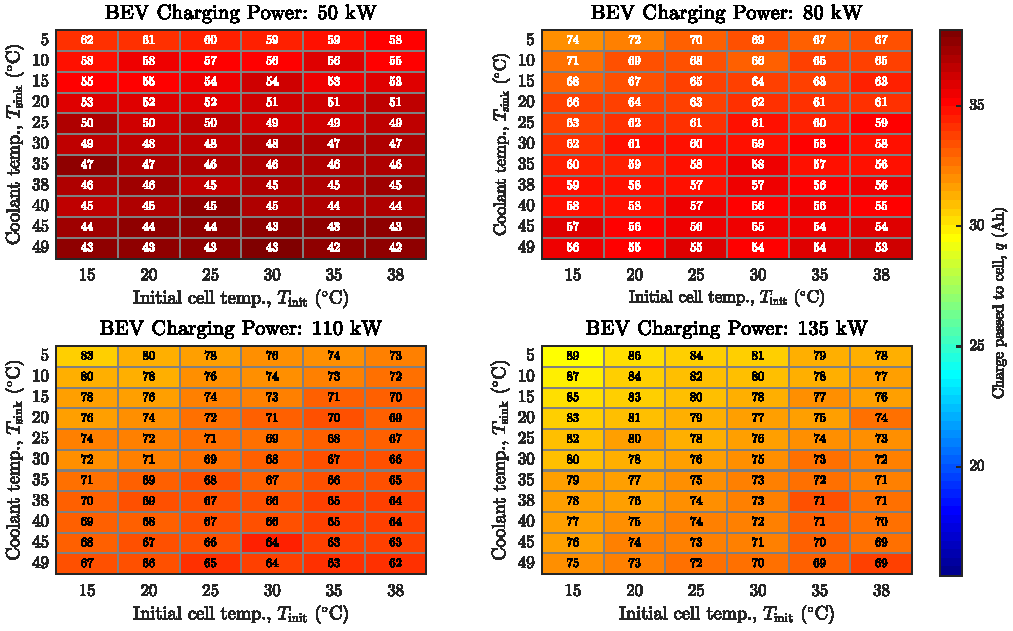
\includegraphics[width=\textwidth]{fig_generate_heatmap_BEV}
        \caption[Optimal cell layer configurations for the \gls{bev}, presented for a range of fast charging powers and thermal conditions]{Optimal cell layer configurations for the \gls{bev}, presented for a range of fast charging powers and thermal conditions\footnotemark.}
        \label{fig:fig_generate_heatmap_BEV}
        \mpfootnotes[1]
        \footnote{This figure was created by Ian Campbell who asserts copyright,
            with  intellectual  contributions  from  and   the  right  to  use  asserted  by
        Krishnakumar Gopalakrishnan.}
    \end{minipage}
\end{figure}

\begin{figure*}[!bp]
    \begin{minipage}[t]{\textwidth}
        \centering 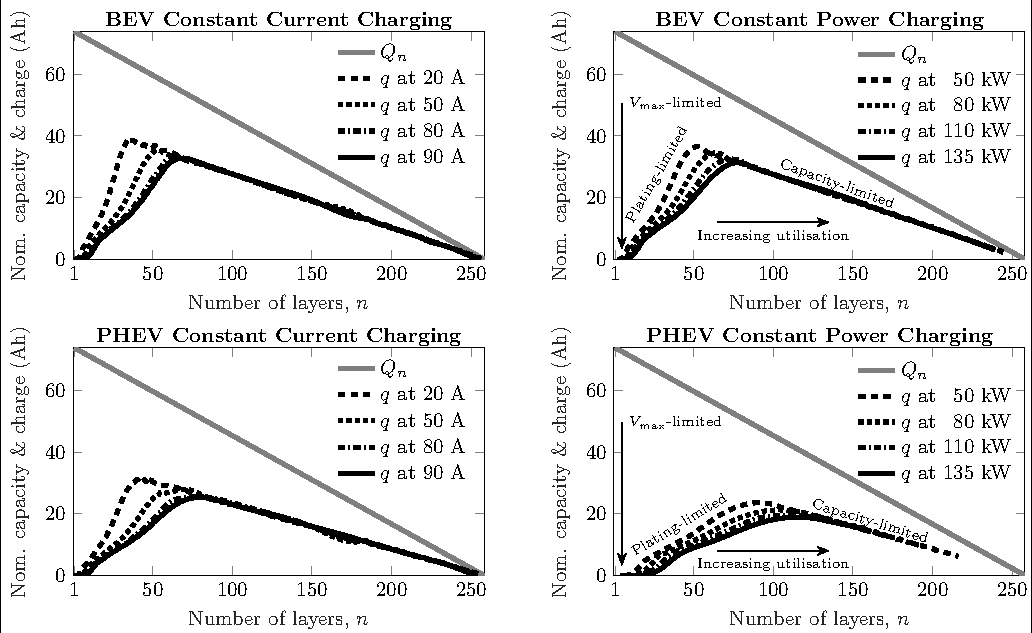
\includegraphics[width=\textwidth,trim=4 2 3 4,clip]{fig_capacity_quadrants.pdf}
        \caption[The plots  in the right  column show the nominal  cell capacity and  charge passed
        during \gls{xeV} \gls{cp} charging. Increased rate capability and cell utilisation are positively
        correlated with  $n$, while the  maximum-$q$ layer  configuration clearly shifts  to higher
        values  of $n$  with  increasing charging  powers.  The  plots in  the  left column  depict
        galvanostatic charging scenarios  at various currents to highlight the  similarity with the
        \gls{cp}  process.  All  data  obtained  at  $T_\text{init}  =$  \SI{25}{\degreeCelsius},
        $T_\text{sink} =$ \SI{25}{\degreeCelsius}.]{The plots  in the right  column show the nominal  cell capacity and  charge passed
            during \gls{xeV} \gls{cp} charging. Increased rate capability and cell utilisation are positively
            correlated with  $n$, while the  maximum-$q$ layer  configuration clearly shifts  to higher
            values  of $n$  with  increasing charging  powers.  The  plots in  the  left column  depict
            galvanostatic charging scenarios  at various currents to highlight the  similarity with the
            \gls{cp}  process.  All  data  obtained  at  $T_\text{init}  =$  \SI{25}{\degreeCelsius},
        $T_\text{sink} =$ \SI{25}{\degreeCelsius}\footnotemark.}\label{fig:fig_CapacityQuadrants}
        \mpfootnotes[1]
        \footnote{This figure was created by Ian Campbell who asserts copyright,
            with  intellectual  contributions  from  and   the  right  to  use  asserted  by
        Krishnakumar Gopalakrishnan.}
    \end{minipage}
\end{figure*}

\begin{figure}[!bp]
    \begin{minipage}[t]{\textwidth}
        \centering
        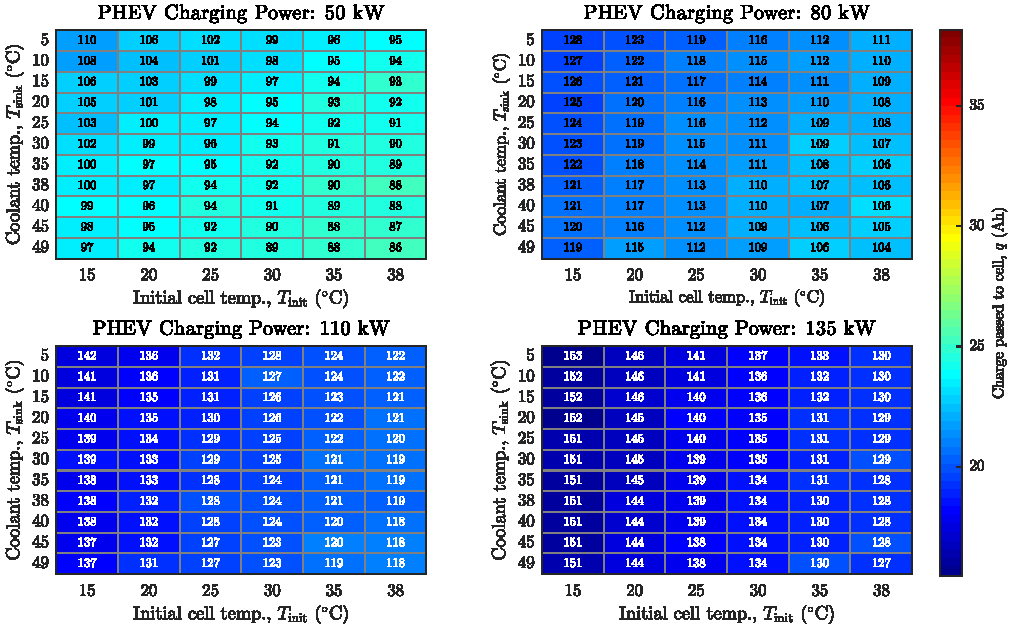
\includegraphics[width=\textwidth]{fig_generate_heatmap_PHEV}
        \caption[Optimal cell  layer configurations for  the \gls{phev},  presented for a  range of
        fast charging powers and thermal conditions]{Optimal cell  layer configurations for  the \gls{phev},  presented for a  range of
        fast charging powers and thermal conditions\footnotemark.}
        \label{fig:fig_generate_heatmap_PHEV}
        \mpfootnotes[1]
        \footnote{This figure was created by Ian Campbell who asserts copyright,
            with  intellectual  contributions  from  and   the  right  to  use  asserted  by
        Krishnakumar Gopalakrishnan.}
    \end{minipage}
\end{figure}
